\setcounter{subsection}{4}
\subsection{Устойчивость выразимых предикатов при автоморфизмах интерпретаций.}

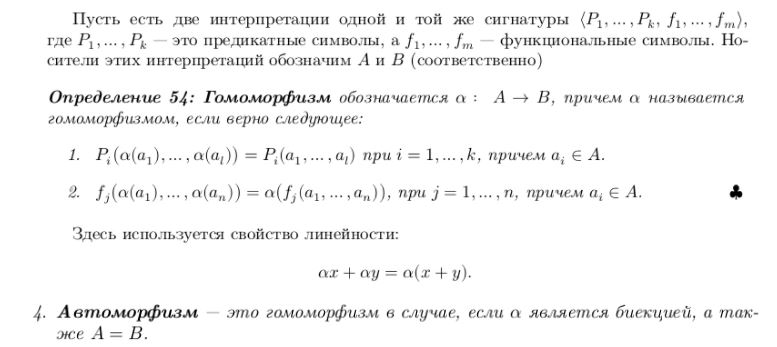
\includegraphics[width=0.95\textwidth]{images/1.5_def}

k-местный предикат P - устойчивыq относительно $\alpha$, если

$P(\alpha(m_1), \dots , \alpha(m_k)) \Leftrightarrow P(m_1, . . . ,m_k)$
для любых элементов $m_1, \dots, m_k \in M$. Далее, k-местная функция f называется \emph{устойчивой} относительно $\alpha$, если
$f(\alpha(m_1), \dots, \alpha(m_k)) = \alpha(f(m_1, \dots ,m_k))$.

\textbf{Теорема}. Любой предикат, выразимый в данной интерпретации, устойчив относительно её автоморфизмов.

$\blacktriangle$
Проведём доказательство этого (достаточно очевидного) утвер-
ждения формально.
Пусть $\pi$ — некоторая оценка, то есть отображение, ставящее в соответствие всем индивидным переменным некоторые элементы носителя. Через $\alpha \circ \pi$ обозначим оценку, которая получится, если к значению каждой переменной применить отображение $\alpha$; другими
словами, $\alpha \circ \pi (\xi)$ для любой переменной $\xi$.

Первый шаг состоит в том, чтобы индукцией по построению терма t доказать такое утверждение: значение терма t при оценке $\alpha \circ \pi$ получается применением $\alpha$ к значению терма t при оценке $\pi$: $[t](\alpha \circ \pi) = \alpha([t](\pi))$.

Для переменных это очевидно, а шаг индукции использует устойчивость всех функций интерпретации относительно $\alpha$. Теперь индукцией по построению формулы $\varphi$ легко доказать такое утверждение: $[\varphi](\alpha \circ \pi) = [\varphi](\pi)$

Мы не будем выписывать эту проверку; скажем лишь, что взаимная однозначность $\alpha$ используется, когда мы разбираем случай кванторов. (В самом деле, если с одной стороны изоморфизма берётся какой-то объект, то взаимная однозначность позволяет взять соответствующий ему объект с другой стороны изоморфизма.)
$\blacksquare$

\subsection{Теорема Гёделя о полноте исчисления предикатов: расширение любого непротиворечивого множества до полного и экзистенциально полного.}

\textbf{Теория} - любое множество замкнутых формул (то есть формул, не имеющих параметров). \textbf{Модель теории} - это любая интерпретация, в которой все формулы из данной теории истинны. \textbf{Совместная теория} - теория, имеющая модель. Теория \textbf{противоречива}, если из нее выводится противоречие, и \textbf{непротиворечива} иначе.

\par
\textbf{Теорема Гёделя, о полноте исчисления предикатов}:
Если $\varphi$ общезначима, то она выводима в исчислении предикатов.
Пользуясь данной терминологией, можно сформулировать теорему, из которой будет следовать теорема Гёделя.

\textbf{Теорема}: Если теория непротиворечива, то она совместна (имеет модель).

\textbf{Доказательство:} 1. Мы хотим расширить не противоречивую Г так, чтобы она была полной (если $\varphi$ - замкнутая формула, то Г $ \vdash \varphi$ или  Г $ \vdash \neg \varphi$) и экзистенциально полной (т.е. если Г $ \vdash \exists x \varphi$, то Г $ \vdash \varphi(t/x)$, где t - замкнутый терм.

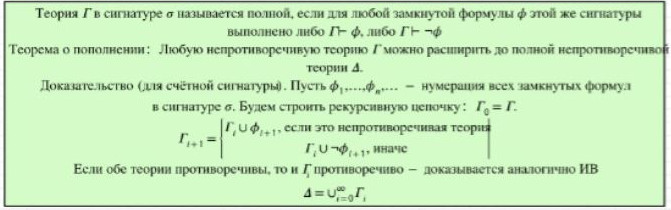
\includegraphics[width=13cm]{images/1.5_m1}

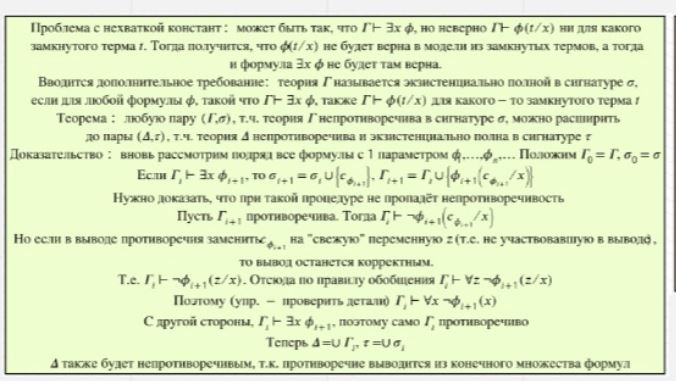
\includegraphics[width=13cm]{images/1.5_m2}

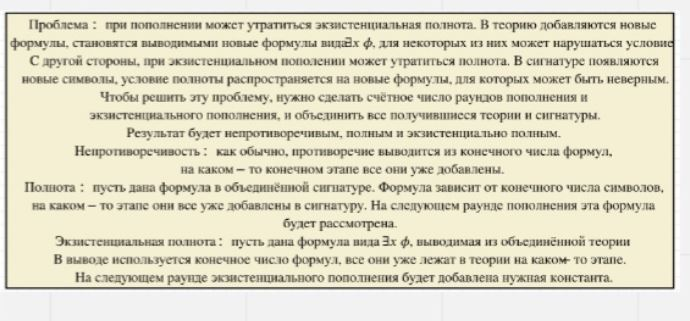
\includegraphics[width=13cm]{images/1.5_m3}

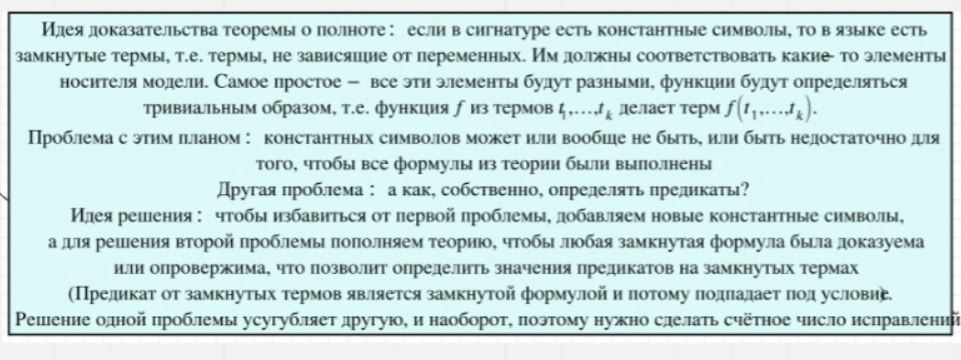
\includegraphics[width=13cm]{images/1.5_full}

\textbf{Лемма 9}.
Любую непротиворечивую теорию можно расширить до непротиворечивой, полной и экзистенциально полной теории.

Доказательство было приведено выше.

\subsection{Теорема Гёделя о полноте исчисления предикатов: построение модели из замкнутых термов у любого непротиворечивого, полного и экзистенциально полного множества.}

\textbf{Лемма 10}.

Любая непротиворечивая, полная, экзистенциально полная теория совместна, то есть имеет модель.

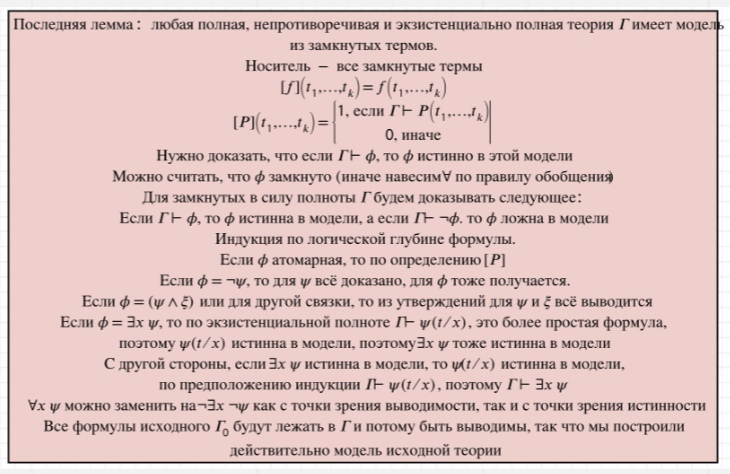
\includegraphics[width=13cm]{images/1.5_full2}\\

\subsection{Представимость конечных последовательностей в арифметике при помощи $\beta$-функции Гёделя.}

\textbf{Лемма 1}:\\

$\forall n \quad \forall c \quad \exists b > c$ такое, что $b + 1,  2b + 1, \dotsc, nb + 1$ - взаимно просты.\\

Рассмотрим $b = n!$.

Тогда возьмем произвольные различные $k$ и $m$ от $1$ до $n$. $gcd(kb + 1, mb + 1) = d > 1 \Rightarrow (k - m)b$ делится на $d$.

Значит т.к. $b = n!$ и $k - m < n$, получаем, что любой простой делитель числа $(k - m)b$ должен быть строго меньше $n$.\\

У $d$ есть простой делитель $p < n$.

$mb + 1$ делится на $p$.

$mb + 1 - m*n!$ делится на $p \Rightarrow d = 1$ 
\\

\textbf{Лемма 2.}\\

$\forall (x_1, \dotsc, x_n) \quad\exists a, b \quad \forall i : a \equiv x_i \quad mod (b_i + 1)$\\

\textbf{Док-во:}\\

Выберем по Лемме 1 $b > max\{x_i\}$.\\

Тогда нужное $a$ найдётся по китайской теореме об остатках: Если натуральные числа $a_1, \dotsc, a_n$  попарно взаимно просты, то для любых $r_1, \dotsc, r_n$ таких, что $0 \leq r_i < a_i$ при всех $i : 0, \dotsc, n$ найдется число, которое при делении на $a_i$ дает остаток $r_i$ при всех $i$. Более того, если найдутся два таких числа, то они будут сравнимы по модулю $a_1 \cdot \dotsc \cdot a_n$.\\

Положим $\beta(a, b, i) = a \quad mod (bi + 1)$

$\beta$ арифметична: $r = x \quad mod(q) \Leftrightarrow r < q$ и $\exists s: x = sq + r$.